\question{Насыщение перехода}

\begin{figure}[h]
	\center
	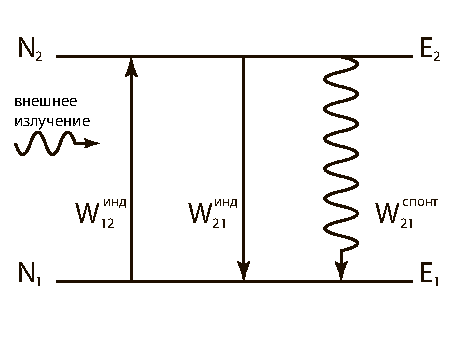
\includegraphics[width=.4\textwidth]{06_01}
\end{figure}

Скорость заселения верхнего уровня
\[
	\frac{dN_2}{dt} = W^\text{и}_{12} N_1 - W^\text{и}_{21} N_2 - 
    	W^\text{сп}_{21} N_2
\]

Под насыщеным переходом внешнего излучения понимается зависимость коэффициента 
поглощения слабого сигнала при воздействии на среду внешним излучением.

Выясним зависимость \( \D N = N_2 - N_1 \). \\
С одной стороны: \( I = I_0 \exp(-\alpha x) \) \\
C другой стороны: \( dI = W_{12}(n_2 - n_1 ) h\nu dx \)
\[ 
	dI = -\alpha I dx
\]
\[
	\alpha \sim n_2 - n_1 \sim N_2 - N_1 \sim \D N 
\]
\[
\begin{array}{c}
	W^\text{и}_{12} = B_{12} \rho_\nu \\
    W^\text{и}_{21} = B_{21} \rho_\nu \\
    B_{12} = B_{21} \rightarrow W^\text{и}_{12} = W^\text{и}_{21} = W \\
    W^\text{сп}_{21} = A_{21} = \frac{1}{\tau}
\end{array} 
\]
\[
	\frac{dN_2}{dt} = WN_1 - WN_2 - \frac{N_2}{\tau};\quad
    \frac{dN_2}{dt} = -W\D N - \frac{N_2}{\tau}
\]
\[
	\left\{ \begin{array}{c}
    	\D N = N_2 - N_1 \\
        N = N_2 + N_1 
    \end{array} \right.
\]
\[
	\D N + N = 2N_2;\quad
    N_2 = \frac{\D N + N}{2}
\]
\[
	\frac{d}{dt}\left( \frac{\D N}{2} + \frac{N}{2} \right) = -W\D N - 
    	\frac{\D N}{2\tau} - \frac{N}{2\tau}
\]

Квазистационарный случай: \( \D N = const \), тогда 
\( \cfrac{d}{dt}(\D N) = 0 \). Получим:
\[
	-\D N\left( 2W + \frac{1}{\tau} \right) - \frac{N}{\tau} = 0
\]
\[
	\D N = \frac{-N}{1+2W\tau}
\]

Разность населённостей энергетических уровней зависит от: \\
1) времени жизни в возбужденном состоянии (\( \tau \)) \\
2) от объёмной плотности (\( W \))